%% ijbm_main.tex -- International Journal of Biological Macromolecules (Elsevier) submission format of
%% manuscript_short/grip_finding.tex. Text from the source except the rule section (44_rule_test, author decision 2026-11-24)
%% and the consistency edits listed in ../manuscript_carbpol/JOURNAL_RULES.md; journal rules there.
%% Build: pdflatex, bibtex, pdflatex x2.
\documentclass[preprint,12pt]{elsarticle}

\usepackage{amsmath,amssymb}
\usepackage{booktabs}
\usepackage{array}
\usepackage{siunitx}
\usepackage{graphicx}
\usepackage{lineno}
\usepackage{rotating}
\usepackage{setspace}% double spacing: IJBM length guidance is in double-spaced pages (unofficial source)
\usepackage[hidelinks]{hyperref}
\graphicspath{{figures/}}
\sisetup{group-separator={\,},group-minimum-digits=4}
\newcommand{\pend}[1]{\textbf{[PENDIENTE: #1]}}

\journal{International Journal of Biological Macromolecules}

\begin{document}

\begin{frontmatter}

\title{Fixed and variable sugar contacts at the subsites of starch-degrading enzymes: a
structural basis for processing functionalised starch}

\author[a,b]{Aldo F. Combariza\corref{cor1}}
\ead{aldo.combariza@unisucre.edu.co}
\cortext[cor1]{Corresponding author.}
\affiliation[a]{organization={Grupo de Investigaci\'{o}n {\itshape in silico},
  Departamento de Biolog\'{\i}a y Qu\'{\i}mica, Universidad de Sucre},
  addressline={Carrera 28 No.\ 5-267},
  city={Sincelejo},
  state={Sucre},
  country={Colombia}}
\affiliation[b]{organization={Doctorado en Ciencias F\'{\i}sicas, Sistema Universitario Estatal del Caribe (SUE Caribe)},
  country={Colombia}}

\begin{abstract}
Functionalised starches, carrying hydroxypropyl, acetyl, octenyl-succinyl or carboxymethyl
groups on O2, O3 or O6 of their glucose units, are processed and analysed
with amylolytic enzymes, but where in the enzyme a substituted glucose unit can sit is not
known in general. We assembled 637 Protein Data Bank entries of 14 starch-active CAZy
families, assigned every density-supported sugar unit to its subsite, and classified every
residue within 4.0~\AA{} of it by kind of contact: side-chain hydrogen bond, aromatic or
aliphatic. In GH13 and GH31, all 36 positions contacted in at least 20\% of
the entries at subsites $-3$ to $+3$ were analysed, with residue identity counted once per
group of proteins sharing 50\% sequence identity (modal fraction $m$).
Of the 13 hydrogen-bonding positions at subsites $-1$ and $+1$, 11 carry one residue type
in every lineage ($m = 1$). Aromatic positions keep an aromatic ring more often than their
identity. Aliphatic positions, and positions of every kind at the outer subsites, vary
between lineages. Hydrogen-bonding positions are more conserved than aliphatic ones by 0.33
(permutation test, $p = 0.003$), robust to class assignment, held-out proteins and the hydrogen-bond definition. Read atom by atom, O2, O3 and O6 at subsite $-1$ and O3 at
$+1$ are held by fixed residues, the GH13 oxygens at $-2$ and $+2$ by variable residues, and
O6 and the outer subsites are mostly free. This map agrees with published products and
kinetics of phosphorylated, hydroxyethylated and O-methylated substrates in 19 of 21
subsite--oxygen cells.
\end{abstract}

%% Graphical abstract: Elsevier specification 1328 x 531 px minimum (5:2, w x h), 300 dpi,
%% TIFF/EPS/PDF/MS Office; uploaded as a separate file in Editorial Manager.
\begin{graphicalabstract}
\fbox{\parbox[c][5.2cm][c]{13cm}{\centering \pend{graphical abstract, to be prepared by the
author; 1328\,$\times$\,531 px minimum, 300 dpi}}}
\end{graphicalabstract}

%% Highlights are in ijbm_highlights.tex (uploaded as a separate Word file).

\begin{keyword}
Starch-degrading enzymes \sep Glycoside hydrolase \sep Subsite \sep Functionalised starch
\sep Protein--carbohydrate interaction \sep Residue conservation \sep Protein Data Bank
\end{keyword}

\end{frontmatter}

\linenumbers
\doublespacing

\section{Introduction}

Starch is modified chemically for engineering uses: hydroxyl groups at O2, O3 and O6 of its
glucose units are etherified or esterified with hydroxypropyl, carboxymethyl, acetyl or
octenyl-succinyl groups, which change its solubility, paste behaviour and emulsifying
capacity~\citep{Masina2017,Chen2015,Altuna2018}. Amylolytic enzymes act on these products,
and enzymatic digestion followed by analysis of the released fragments is a standard route
to where the substituents lie along the chain~\citep{Richardson2003,Mischnick2010,Zhao2012}.
A substituent changes what an enzyme releases: pancreatic $\alpha$-amylase gives different
hydrolysis products from modified and unmodified tapioca starch~\citep{Conway1976}. The
extent of hydrolysis and the product profile therefore depend on which substituted glucose
units an enzyme accepts at each of its subsites, and through which oxygen. This has been
measured for particular enzymes and substituents, not in general.

Native starch is the plant's storage carbohydrate: two glucose polymers, amylose (mostly
linear, $\alpha(1\!\to\!4)$-linked glucose) and amylopectin (the same linkage, with
$\alpha(1\!\to\!6)$ branch points). The enzymes that break it down are sorted by CAZy~\citep{Drula2022}
into families by sequence similarity, not by function: the same job, cutting an
$\alpha(1\!\to\!4)$ bond in the middle of the chain, is carried out by families with
different folds and catalytic machinery (GH13; GH57 and GH119, which form one clan;
GH126)~\citep{Janecek2014}. Within a family, two catalytic carboxylic acids do the
chemistry: in a retaining mechanism, one is the nucleophile that attacks the sugar, the
other the acid/base that first protonates the leaving group and then activates the water
that completes the reaction. The residues around this pair define subsites, numbered from
the bond that is cut: negative towards the non-reducing end of the chain, positive towards
the reducing end~\citep{Davies1997}.

Because the catalytic chemistry is fixed within a family, what distinguishes one enzyme
from another of the same family is usually described as the set of residues at the
other subsites~\citep{Davies1995}. In GH13, sequence comparison has long identified the
conserved sequence regions that carry the catalytic triad, an invariant arginine and two
histidines at the catalytic subsite~\citep{MacGregor2001,Janecek2014}, and surveys of
deposited glycoside hydrolase complexes have been used to show how these enzymes hold the
sugar near the transition state~\citep{Quirke2020}. Structural comparisons of the residues
around the bound sugar have mostly been made one structure, or a few, at a time. Which residues around the bound sugar are fixed across the many independently solved
structures of a family, which ones change, and what decides the difference, has not been
asked at the scale of hundreds of structures.

The question asked here is the one a design map for processing functionalised starch
needs: at each subsite of the starch-degrading enzymes, which contacts with the sugar are
fixed across lineages, and which vary. To answer it, we built an experimental database of
637 PDB entries covering 14 starch-active CAZy families, superposed every structure of each family on one reference, and recorded, for
every bound sugar unit, its position along the chain, the protein residues within
4.0~\AA{} of it, and the kind of contact each residue makes.

% Figure 1 (protein overview, chemistry of substituted starch): being produced, see figures/candidates/fig1_protein/
\begin{figure}[t]
\centering
\fbox{\parbox[c][4cm][c]{0.9\linewidth}{\centering \pend{Figure 1: enzyme overview and chemistry of
functionalised starch, being prepared}}}
\caption{\pend{caption of Figure 1}}
\label{fig:overview}
\end{figure}

\section{Materials and methods}

\subsection{Database and superposition}
Every PDB entry of the 14 families was read
with gemmi~\citep{Wojdyr2022}; every non-water, non-standard residue was registered with
its fit to the experimental electron density (the real-space correlation coefficient,
RSCC; $\mathrm{RSCC}\ge0.80$ is called density-supported here). Residue numbers differ
between structures of the same protein, so every chain was mapped through
SIFTS~\citep{Velankar2013} to one UniProt numbering, and every structure of a family was
superposed on one reference by its core C$\alpha$ atoms around the catalytic site
(Kabsch fit~\citep{Kabsch1976}). The one assumption of this step is that the core
C$\alpha$ atoms of a family occupy equivalent positions in all its members. This
superposition itself exposed a curation error: eight cryo-EM entries listed under GH63
failed to fit the family core at all and were found, on inspection, to be crescentin
filaments -- a bacterial cytoskeletal protein unrelated to any carbohydrate-active
enzyme -- wrongly filed under this family; they were removed, leaving 637 entries.

\subsection{Position along the chain}\label{sec:position}
For the five families whose frame carries an
identified catalytic pair (GH13, GH14, GH15, GH31, GH57), every bound sugar unit was
assigned a subsite: the unit nearest the midpoint of the two catalytic carboxylates,
within 4.5~\AA, is subsite $-1$; the rest follow the deposited glycosidic bonds outward.
Every protein residue within 4.0~\AA{} of a unit was named by its position in the
family's reference frame rather than by its author number, so that the same position can
be compared across different proteins. Two properties of a position are kept apart in what
follows: how often it touches the sugar (it is \emph{contacted}) and whether different
proteins carry the same residue type there (it is \emph{conserved}, and \emph{fixed} when
every lineage carries the same residue). For GH13 and GH31
(Section~\ref{sec:rule}), the positions analysed are all reference positions contacted
(4.0~\AA) in at least 20\% of the entries with a sugar unit at any subsite from $-3$ to
$+3$, taken before their residues were examined. Residue identity at each position is read
for every chain from the superposition (C$\alpha$ within 2.0~\AA{} of the reference
C$\alpha$) and counted once per group of proteins sharing at least 50\% sequence identity;
conservation is the modal fraction $m$ of these group votes (eq~\ref{eq:modal}). Engineered
mutants, identified from the \texttt{\_struct\_ref\_seq\_dif} records of each entry, are
removed at the mutated position. Sections~\ref{sec:inhib}--\ref{sec:folds} use an earlier,
stricter selection, positions contacted in at least 80\% of the entries with a unit at a
given subsite, with residues counted per entry; each place where this criterion is used
says so.

\subsection{Kind of contact}\label{sec:methods_contacts}
For each contacted position and each entry, the residue and
the sugar unit were read from the deposited coordinates (model 1, first alternate
conformation). The contact is a side-chain hydrogen bond when a side-chain nitrogen or
oxygen lies within 3.5~\AA{} of a sugar oxygen or nitrogen; a backbone hydrogen bond when
only a main-chain N or O does; apolar otherwise. An apolar contact is aromatic or
aliphatic by the residue that makes it. The class of a position is the kind of contact it
makes in most sequence groups. The one assumption is that a 3.5~\AA{} N/O--N/O distance
stands for a hydrogen bond; no angle is tested in the main count, and no hydrogens are
placed. The sensitivity of the result to this definition (cut-offs of 3.2 and 4.0~\AA, and
3.5~\AA{} with both heavy-atom angles at least 90$^\circ$) is reported in
Section~\ref{sec:rule}. Figure~\ref{fig:active} shows two entries drawn with the same criterion:
1G94 (GH13, \emph{Pseudoalteromonas haloplanktis} $\alpha$-amylase, 1.74~\AA; the sugar units
drawn at subsites $-1$, $+1$ and $+2$ have RSCC 0.95--0.97) and 3WEO (GH31, sugar beet
$\alpha$-glucosidase, 1.45~\AA; RSCC 0.99); residues are labelled in the reference numbering
(1AMY for GH13, 2QMJ for GH31), and the classes are those of Table~\ref{tab:rule}.

\subsection{Glucose oxygens and their protein partners}\label{sec:methods_map}
The units are those of Section~\ref{sec:rule} (RSCC $\ge0.80$, subsites $-3$ to $+3$) in GH13,
GH31, GH14 and GH15: glucose and the glucose-like rings of inhibitors (modified glucose,
cyclitol and iminosugar rings). Atoms were labelled from the bonded graph of each ring, not
from atom names, because multi-ring components carry suffixed names: C1 is the anomeric (or
pseudo-anomeric) carbon, the ring is walked C1--C2--C3--C4--C5, C6 is the exocyclic carbon on
C5, and O2, O3, O4 and O6 are the exocyclic heteroatoms (O, N, F or S) on C2, C3, C4 and C6;
a C1 heteroatom bonded to another ring is the glycosidic atom and is counted as O4 of the
next unit. A unit whose configuration at C2--C4 is opposite to $\alpha$-D-glucose was
excluded as an epimer, as were rings named as other sugars and rings without an unambiguous
O5 (15 units). An oxygen is \emph{held} when a protein N or O of the deposited asymmetric unit
lies within 3.5~\AA{} of it (waters are not partners). The partner is \emph{invariant} when it
is a side chain at a reference position whose modal fraction $m$ (eq~\ref{eq:modal}) is 1 over at
least three sequence groups in GH13 and GH31, or over both groups in GH14 and GH15; here $m$ is
counted over all ligand-bound entries of the family, mutants removed. The open surface of each
oxygen was computed by the Shrake--Rupley method (480 points per atom, probe 1.4~\AA, Bondi
radii, no hydrogens, waters removed) in the complex and in the ligand alone. The properties
were aggregated from atom to entry (an entry has the property when at least half of its units
at that subsite do), from entry to 50\% sequence group (at least half of its entries), and
from group to cell (subsite $\times$ oxygen). A cell is held when at least half of the groups
hold the oxygen; it is then INV (fixed) when at least half of the groups hold it by an
invariant side chain, VAR (variable) when the remaining side-chain partners are variable, and
MC when only main-chain atoms hold it. A cell that is not held is EXP (free, exposed) when the
median open surface is at least 5~\AA$^2$ and at least 25\% of the surface of the same atom in
the ligand alone, and BUR (free, buried) otherwise. Script:
\texttt{scripts/analysis/a45\_hydroxyl\_map.py}; output:
\texttt{resultados/analysis/45\_hydroxyl\_map/}.

For the comparison with experiment (Table~\ref{tab:mapexp}), published limit products and
kinetics of substituted substrates were read onto subsites with the standard rule for
products~\citep{Davies1997}: when an endo-acting enzyme cuts, the new reducing-end residue sat at
$-1$ and the new non-reducing-end residue at $+1$, so a substituted residue at position $k$ from
the reducing end of a limit product of length $n$ was tolerated at subsite $-k$ (and at
$+(n-k+1)$ when that end is not an original chain end), and a linkage left uncut inside a limit
product marks a non-productive placement. Each cell then carries a prediction: INV, substituent
not tolerated; EXP, tolerated; VAR, tolerance depending on the enzyme (agreement when enzymes of
the family differ or at least one tolerates it). MC and BUR cells make no prediction. Every
literature result is labelled by what was read: full text (FT) or abstract (ABS); the reading
of products onto subsites is ours unless the authors state it.


\section{Results and discussion}

\subsection{Which contact positions keep their residue across lineages}\label{sec:rule}

\paragraph{Positions and counting} To avoid choosing positions after seeing their residues,
every reference position contacted (4.0~\AA) in at least 20\% of the entries with a sugar
unit at a subsite from $-3$ to $+3$ was taken: 17 positions in GH13 and 19 in GH31, the five
catalytic residues among them. Residue identity at each position was read for every chain from
the superposition (a residue belongs to a reference position when its C$\alpha$ lies within
2.0~\AA{} of the reference C$\alpha$), not only for chains whose residue touches the sugar, and
was counted once per group of proteins sharing at least 50\% sequence identity (29 groups in
GH13, 6 in GH31). Engineered mutants were removed at the mutated position (1QI5, 5TD4, 9UNS,
9XG6 at Asp289; 7WJC, 7WJF at Asp542; 3PHA, 3BLP, 3DHP, 3OLD, 3OLE, 3OLG, 3OLI, 1UA7 and 8CQF at
the positions they alter, from the \texttt{\_struct\_ref\_seq\_dif} records). The class of a
position is the contact kind made in most groups (H, side-chain hydrogen bond; Ar, apolar
contact by an aromatic residue; Al, apolar contact by an aliphatic residue). Conservation of a
position is the modal fraction
\begin{equation}
m = \frac{\max_a n_a}{\sum_a n_a},
\label{eq:modal}
\end{equation}
where $n_a$ is the number of group votes for residue type $a$ (a group whose members differ
splits its vote). For GH13 Lys182: Lys 9.5, Arg 2.5, His 2, Gln 1 of 15 groups,
$m = 9.5/15 = 0.63$. For aromatic positions the aromatic fraction (Phe, Tyr, Trp, His) is also
given.

\paragraph{What is read off} Table~\ref{tab:rule} lists the 36 positions (two
catalytic subsites are drawn in Fig.~\ref{fig:active}); 35 have a majority class
(17 H, 10 Ar, 8 Al) and one, GH31 Thr544, has none. Of the 13 hydrogen-bonding positions that contact a ring at subsite $-1$
or $+1$, eleven carry one residue type in every group ($m = 1$): in GH13 the catalytic Asp179,
Glu204 and Asp289 and the non-catalytic Arg177 and His92, with His288 at 0.97 (one natural Gln,
6SAO); in GH31 the catalytic Asp443 and Asp542 and the non-catalytic Asp327, His600, Asp203 and
Arg526. The one hydrogen-bonding position at $-1$/$+1$ that varies is the GH13 position of
Gly183 ($m = 0.50$): it is His in the eight groups where it contacts the sugar and Gly, Tyr, Glu
or Met where it does not. The ten aromatic positions keep an aromatic ring more often than
their identity (aromatic fraction 0.41--1.00, identity 0.31--1.00). The aliphatic positions vary
(GH13 Phe180 position: Ala, Val, Thr, Leu, Phe, Tyr, Met, $m = 0.24$; GH31 Ile328, $m = 0.50$),
with two exceptions: GH31 Met444 ($m = 0.83$) and GH13 Thr207, which is Lys in both of
its only two groups. At the outer subsites ($-3$, $-2$, $+2$, $+3$),
hydrogen-bonding positions vary as much as the aliphatic ones: GH13 Lys182 0.63, Met52 0.41,
Gln294 0.80, GH31 Asn207 0.50.

\paragraph{The test} Table~\ref{tab:tests} gives the differences in mean $m$ between classes
and their significance by permutation of the class labels over positions (10\,000
permutations; 95\% intervals from 2\,000 bootstrap resamples of the sequence groups). The
hydrogen-bonding positions are more conserved than the aliphatic ones by 0.33 (all 35
positions, $p = 0.003$) and by 0.28 without the catalytic residues ($p = 0.015$). The result
holds when the class is taken from the reference structure alone instead of from the groups
($p = 0.005$--0.016), when the class is assigned on a random half of the groups and conservation
measured on the other half (positive in all 1\,000 splits; median 0.30, 95\% range
0.17--0.41), on 98 entries of 37 groups never seen with a bound sugar ($+0.31$, $p = 0.007$),
and for hydrogen-bond cut-offs of 3.2, 3.5 and 4.0~\AA{} with or without an angle criterion
($p = 0.003$--0.040). Aromatic positions keep an aromatic ring more often than aliphatic
positions keep their residue ($+0.33$, $p < 0.001$). Hydrogen-bonding and aromatic positions do
not differ significantly ($+0.18$, $p = 0.052$; held-out groups $+0.08$, $p = 0.23$). Within the
hydrogen-bonding class, positions at $-1$/$+1$ are more conserved than positions that contact
only the outer subsites (0.96 against 0.59, 13 and 4 positions, $p = 0.0015$); at the outer
subsites, hydrogen-bonding and aliphatic positions do not differ ($-0.09$, $p = 0.67$).

\paragraph{The statement the data support} The residues whose side chains hydrogen-bond the two
rings on either side of the cut are fixed in every lineage; aromatic residues at the same
subsites are kept as aromatic rings, less strictly as the same residue; aliphatic residues at
these subsites, and residues of every kind at the outer subsites, change between lineages.
Conservation is therefore set jointly by where a residue touches the sugar and by the kind of
contact it makes, not by the kind of contact alone.

\paragraph{Limits} GH31 rests on six groups, three of them not $\alpha$-glucosidases (an
$\alpha$-xylosidase and an $\alpha$-1,4-glucan lyase carry the Trp539$\to$Phe, Phe575$\to$His
and Met444$\to$Trp changes and, with the lyase, Ile364$\to$Asn); within the three
$\alpha$-glucosidases only Ile328, Tyr299 and five outer positions vary. Only four
hydrogen-bonding positions lie at the outer subsites. Hydrogen bonds are judged from heavy
atoms; aromatic stacking from residue type, not from ring geometry.

\begin{figure}[t]
\centering
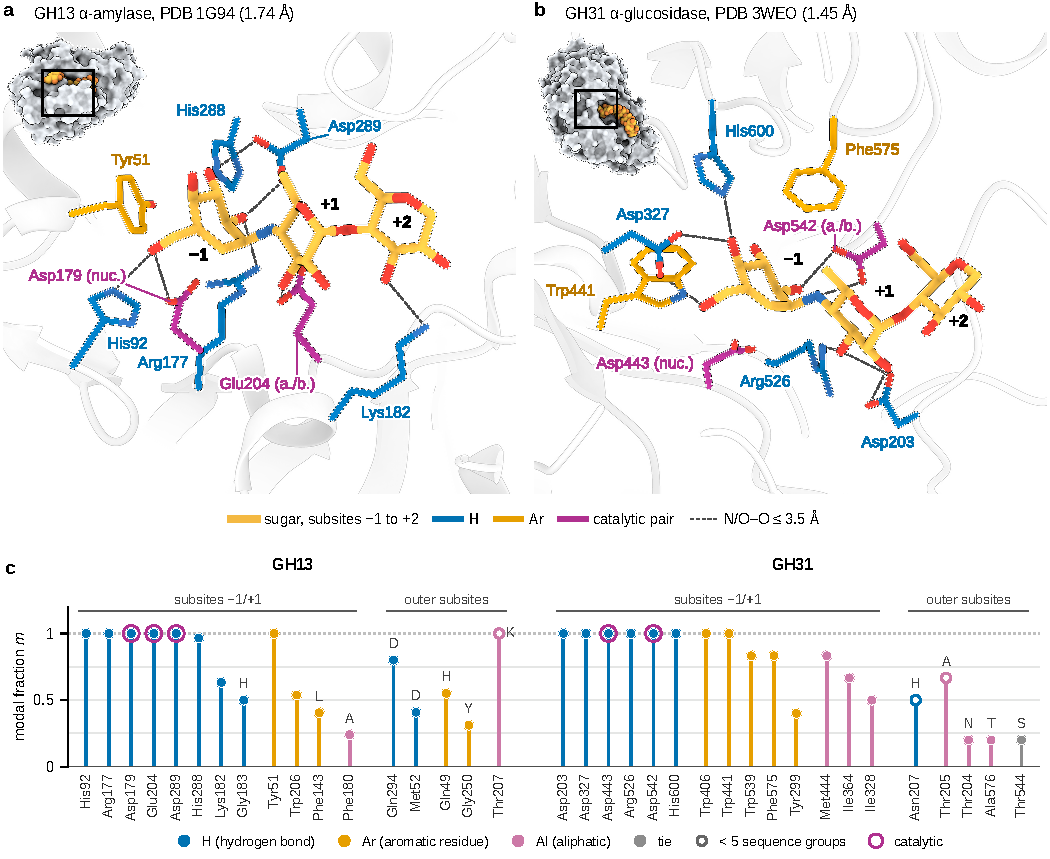
\includegraphics[width=\linewidth]{fig2_active_site.pdf}
\caption{Contacts at the catalytic subsites of (a) GH13 $\alpha$-amylase (PDB 1G94) and (b) GH31
$\alpha$-glucosidase (PDB 3WEO): sugar gold, subsites numbered; side chains coloured by contact
(blue H, orange Ar, pink Al; catalytic pair magenta); dashes, H-bonds $\le$3.5~\AA. (c)
Conservation $m$ of each position (one vote per 50\% sequence group) by class.}
\label{fig:active}
\end{figure}

\begin{table}[p]
\centering\renewcommand{\baselinestretch}{1}\scriptsize\setlength{\tabcolsep}{3pt}
\caption{Every reference position contacted in at least 20\% of the entries with a sugar unit at subsites $-3$ to $+3$ (GH13 reference 1AMY/1BG9, GH31 reference 2QMJ). Class: contact kind made in most sequence groups (H, side-chain hydrogen bond; Ar, aromatic apolar; Al, aliphatic apolar). Groups: proteins sharing $\ge$50\% sequence identity; residues: votes per group (a mixed group splits its vote); $m$: modal fraction (eq~\ref{eq:modal}); Arom.: aromatic fraction. $^\ast$catalytic residue. Engineered mutants removed. Source: \texttt{44\_rule\_test/C\_identity\_T20.tsv}.}
\label{tab:rule}
\begin{tabular}{lllrp{4.6cm}rr}
\toprule
Class & Family & Position (subsites) & Groups & Residues (group votes) & $m$ & Arom.\\
\midrule
H & GH13 & Asp179$^\ast$ ($-$1) & 29 & Asp 29 & 1.00 & 0.00\\
H & GH13 & Asp289$^\ast$ ($+$1,$-$1,$-$2) & 28 & Asp 28 & 1.00 & 0.00\\
H & GH13 & Glu204$^\ast$ ($+$1,$-$1) & 29 & Glu 29 & 1.00 & 0.00\\
H & GH13 & His92 ($-$1) & 29 & His 29 & 1.00 & 1.00\\
H & GH13 & Arg177 ($-$1) & 29 & Arg 29 & 1.00 & 0.00\\
H & GH13 & His288 ($-$1) & 29 & His 28, Gln 1 & 0.97 & 0.97\\
H & GH13 & Gln294 ($-$2) & 15 & Asp 12, Asn 2, Gln 1 & 0.80 & 0.00\\
H & GH13 & Lys182 ($+$1,$+$2) & 15 & Lys 9.5, Arg 2.5, His 2, Gln 1 & 0.63 & 0.13\\
H & GH13 & Gly183 ($+$1) & 16 & His 8, Gly 5, Tyr 1, Glu 1, Met 1 & 0.50 & 0.56\\
H & GH13 & Met52 ($-$2,$-$3) & 22 & Asp 9, Trp 5, Asn 3, Gln 2, Gly 2, Phe 1 & 0.41 & 0.27\\
H & GH31 & Asp203 ($+$1) & 5 & Asp 5 & 1.00 & 0.00\\
H & GH31 & Asp327 ($-$1) & 6 & Asp 6 & 1.00 & 0.00\\
H & GH31 & Asp443$^\ast$ ($-$1) & 6 & Asp 6 & 1.00 & 0.00\\
H & GH31 & Asp542$^\ast$ ($+$1,$+$2,$-$1) & 6 & Asp 6 & 1.00 & 0.00\\
H & GH31 & His600 ($-$1) & 6 & His 6 & 1.00 & 1.00\\
H & GH31 & Arg526 ($+$1,$-$1) & 5 & Arg 5 & 1.00 & 0.00\\
H & GH31 & Asn207 ($+$3) & 2 & His 1, Asn 1 & 0.50 & 0.50\\
\midrule
Ar & GH13 & Tyr51 ($-$1,$-$2) & 29 & Tyr 29 & 1.00 & 1.00\\
Ar & GH13 & Gln49 ($-$2) & 20 & His 11, Trp 6, Val 2, Glu 1 & 0.55 & 0.85\\
Ar & GH13 & Trp206 ($+$1,$+$2,$+$3) & 13 & Trp 7, Phe 3, Ile 1, Tyr 1, Leu 1 & 0.54 & 0.85\\
Ar & GH13 & Phe143 ($-$1) & 21 & Leu 8.5, Phe 7, His 1, Asn 1, Cys 1, Val 1, Ser 1, Tyr 0.5 & 0.41 & 0.41\\
Ar & GH13 & Gly250 ($+$3) & 8 & Tyr 2.5, Phe 2, Thr 1.5, Ser 1, Glu 1 & 0.31 & 0.56\\
Ar & GH31 & Trp406 ($+$1,$-$1) & 5 & Trp 5 & 1.00 & 1.00\\
Ar & GH31 & Trp441 ($-$1) & 6 & Trp 6 & 1.00 & 1.00\\
Ar & GH31 & Phe575 ($+$1,$+$2,$-$1) & 6 & Phe 5, His 1 & 0.83 & 1.00\\
Ar & GH31 & Trp539 ($-$1) & 6 & Trp 5, Phe 1 & 0.83 & 1.00\\
Ar & GH31 & Tyr299 ($+$1,$-$1) & 5 & Tyr 2, Trp 2, Phe 1 & 0.40 & 1.00\\
\midrule
Al & GH13 & Thr207 ($+$3) & 2 & Lys 2 & 1.00 & 0.00\\
Al & GH13 & Phe180 ($+$1,$-$1) & 29 & Ala 7, Val 7, Thr 6, Leu 4, Phe 3, Tyr 1, Met 1 & 0.24 & 0.14\\
Al & GH31 & Met444 ($+$1,$-$1) & 6 & Met 5, Trp 1 & 0.83 & 0.17\\
Al & GH31 & Ile364 ($-$1) & 6 & Ile 4, Asn 2 & 0.67 & 0.00\\
Al & GH31 & Thr205 ($+$2,$+$3) & 3 & Ala 2, Pro 1 & 0.67 & 0.00\\
Al & GH31 & Ile328 ($-$1) & 6 & Ile 3, Val 1, Leu 1, Met 1 & 0.50 & 0.00\\
Al & GH31 & Ala576 ($+$2,$+$3) & 5 & Thr 1, Gly 1, Phe 1, Ala 1, Leu 1 & 0.20 & 0.20\\
Al & GH31 & Thr204 ($+$3) & 5 & Asn 1, Asp 1, Gln 1, Ile 1, Leu 1 & 0.20 & 0.00\\
\midrule
none & GH31 & Thr544 ($+$3) & 5 & Ser 1, Lys 1, Thr 1, Ala 1, Trp 1 & 0.20 & 0.20\\
\bottomrule
\end{tabular}
\end{table}

\begin{table}[h]
\centering\renewcommand{\baselinestretch}{1}\scriptsize\setlength{\tabcolsep}{3pt}
\caption{Difference in mean modal fraction $m$ between classes (H$-$Al, H$-$Ar) and between the aromatic fraction of Ar positions and $m$ of Al positions (Ar(arom)$-$Al); one-sided $p$ from 10\,000 permutations of the class labels over positions; 95\% interval from 2\,000 bootstrap resamples of sequence groups (conservative, see text). Positions contacted in $\ge$20\% of entries; one vote per 50\% sequence group. Source: \texttt{44\_rule\_test/D\_tests.tsv}.}
\label{tab:tests}
\begin{tabular}{llrrlr}
\toprule
Set & Statistic & $n$ H/Ar/Al & Difference & 95\% interval & $p$\\
\midrule
All positions & H$-$Al & 17/10/8 & +0.33 & [0.12, 0.41] & 0.003\\
All positions & H$-$Ar & 17/10/8 & +0.18 & [0.09, 0.25] & 0.052\\
All positions & Ar(arom)$-$Al & 17/10/8 & +0.33 & [0.09, 0.38] & $<$0.001\\
\addlinespace
Without catalytic & H$-$Al & 12/10/8 & +0.28 & [0.07, 0.36] & 0.015\\
Without catalytic & H$-$Ar & 12/10/8 & +0.13 & [0.03, 0.21] & 0.139\\
Without catalytic & Ar(arom)$-$Al & 12/10/8 & +0.33 & [0.08, 0.39] & $<$0.001\\
\addlinespace
Held-out groups & H$-$Al & 17/10/8 & +0.31 & [0.03, 0.32] & 0.007\\
Held-out groups & H$-$Ar & 17/10/8 & +0.08 & [0.01, 0.16] & 0.233\\
Held-out groups & Ar(arom)$-$Al & 17/10/8 & +0.30 & [0.02, 0.28] & $<$0.001\\
\addlinespace
Outer subsites & H$-$Al & 4/5/6 & -0.09 & [-0.28, 0.06] & 0.672\\
Outer subsites & H$-$Ar & 4/5/6 & -0.09 & [-0.21, 0.10] & 0.665\\
Outer subsites & Ar(arom)$-$Al & 4/5/6 & +0.17 & [-0.08, 0.23] & 0.004\\
\addlinespace
Split halves (1\,000) & H$-$Al & -- & +0.30 (median) & [0.17, 0.41] & $>$0 in 100\%\\
H at $-1$/$+1$ vs outer & H$-$H & 13/4 & +0.37 & -- & 0.0015\\
\bottomrule
\end{tabular}
\end{table}



\subsection{Which glucose oxygens the enzyme holds at each subsite}\label{sec:map}

\paragraph{Problem and data} A substituent sits on O2, O3 or O6 of a glucose unit, so the
question a processing design asks is not which residues are fixed but which oxygens they
hold. The rule of Section~\ref{sec:rule} was therefore read atom by atom. The data are 439
density-supported glucose-like units in 114 entries: GH13, 299 units in 76 entries; GH31, 77 in
17; GH14, 43 in 17; GH15, 20 in 4. In GH13 the subsites $-3$ to $+3$ are represented by 17, 22,
29, 17, 15 and 10 sequence groups; in GH31, subsite $-1$ by 6 groups and $+1$ to $+3$ by 5; GH14
($-2$ to $+2$) and GH15 ($-1$ to $+3$) by two lineages each. For every O2, O3, O4 and O6 the
protein N/O partners within 3.5~\AA, the identity of the residue that provides them and the
open surface of the atom were recorded, and each subsite $\times$ oxygen cell was given one of
five states (Section~\ref{sec:methods_map}).

\paragraph{What is read off} Figure~\ref{fig:map} gives the state of every cell and the fraction of
sequence groups in which the oxygen is held. At subsite $-1$, O2, O3 and O6 are held by
invariant side chains with a median open surface of 0~\AA$^2$ in GH13 (O2 by Asp289 and Arg177,
O3 by Asp289 and His288, O6 by Asp179 and His92, in 28--29 of 29 groups), GH31 (Asp542 and
Arg526; His600; Asp327) and GH15 (Arg305; Arg54; Asp55). In GH14, O6 at $-1$ is held by the
invariant Glu380 and Lys295, but O2 and O3 only by main-chain atoms (MC). At $+1$, O3 is held
by an invariant residue in all four families (GH13 Glu204; GH31 Asp203 and Arg526; GH14
Thr342; GH15 Glu180 and Arg305), and the scissile oxygen, O4 of the $+1$ unit, by catalytic
residues in all four (GH13 Asp289 and Glu204, GH31 Asp542, GH14 Glu186, GH15 Glu179). O2 at $+1$ differs between families: held by a variable residue in GH13 (the
Gly183 position, His in 11 of 28 groups, $m = 0.39$; and Lys182), by the invariant Asp203 in
GH31 and Glu180 in GH15, by main chain in GH14. In GH13, O2 and O3 at $-2$ and at $+2$ are held
only by variable residues (at $-2$, the Gln294 position, $m = 0.60$, and residues with no
structural equivalent in the reference; at $+2$, the Lys182 position, $m = 0.50$), and O6 at
$-2$ by the variable Met52 position ($m = 0.52$), while O6 at $+2$ is free and exposed (median
27~\AA$^2$). The outer subsites are mostly free: GH13 $-3$ (O2, O3, O6 exposed, 14--26~\AA$^2$)
and O6 at $+3$ (33~\AA$^2$; O2 and O3 at $+3$ only by main chain), GH31 $+2$ and $+3$ (O2 and O3,
31--36~\AA$^2$; O6 at $+2$, 12~\AA$^2$), GH15 $+2$ and $+3$ (O2 and O3, 25--42~\AA$^2$; O6 at $+3$,
18~\AA$^2$).

\paragraph{Checks} In the entries whose units are glucose only, GH13 keeps the same states at
$-1$ (O2, O3, O6 fixed; 24 entries, 16 groups), $-2$ (O2, O3, O6 variable; 24 entries, 11
groups) and $+1$ (O3 and O4 fixed; 3 entries), and GH31 at $-1$ (5 entries). Every residue that
makes a cell fixed in GH13 and GH31 is a position with $m = 1$ in Table~\ref{tab:rule}.

\paragraph{Limits} Units at $-1$ and $+1$ are mostly inhibitors: in GH13, 49 of 82 units at $-1$ are
cyclitol or iminosugar rings and 47 of 50 at $+1$ the 4-amino-4,6-dideoxyglucose of
acarbose-type inhibitors; in GH31, 24 of 32 and 16 of 16; in GH15, all. Because that $+1$ ring
lacks O6, there is no density-supported O6 at $+1$ in GH31 and GH15, and only three units carry
it in GH13. A partner is judged by distance alone, with no angle and no hydrogens. EXP means
that the oxygen has open surface in the deposited complex, not that a substituent has room
there. Invariance in GH14 and GH15 rests on two lineages. No glucose unit bearing a
hydroxypropyl, acetyl, octenyl-succinyl or carboxymethyl group, nor any 2-O- or
3-O-substituted glucose, is bound in these families in the PDB; the 18 substituted rings of the
census carry their substituent on O1 or O4 (\texttt{45\_hydroxyl\_map/substituted\_glucose\_in\_census.tsv}).

\paragraph{The map against experiment} Table~\ref{tab:mapexp} sets every cell for which a
positional result with a substituted substrate was found against the prediction of its state.
Of the 21 cells with a prediction (INV, VAR or EXP), 19 agree. All three variable GH13 cells
with data ($-2$ O3, $-2$ O6, $+2$ O3) are cells where the phosphate products of \emph{Bacillus
subtilis}, porcine pancreatic and \emph{Aspergillus oryzae} $\alpha$-amylases
differ~\citep{Takeda1983,TakedaHizukuri1986,Takeda1987}. The two disagreements are both at a fixed
cell of subsite $+1$. In GH15, O2 at $+1$ is held by Glu180 in both lineages of the map (median
9~\AA$^2$ open), yet the O-methyl and deoxy analogues at OH-2 of the reducing unit are hydrolysed
with kinetics virtually unchanged~\citep{Lemieux1996,Bock1987}: O2 at $+1$ is free in the
kinetics. In GH14, O6 at $+1$ is held by the catalytic Glu186 and by Arg188 in both lineages
(three entries), yet sweet-potato $\beta$-amylase cleaves with a 6-phosphorylated residue at
$+1$~\citep{Takeda1987}. Of the four cells without a prediction, GH13 O3 at $+3$ (main chain) carries a
tolerated 3-phosphate, GH13 O6 at $+1$ (buried, three units) a 6-phosphate tolerated by two of
three $\alpha$-amylases, and GH14 O3 at $-1$ (main chain) a 3-phosphate that is not tolerated.

\begin{figure}[t]
\centering
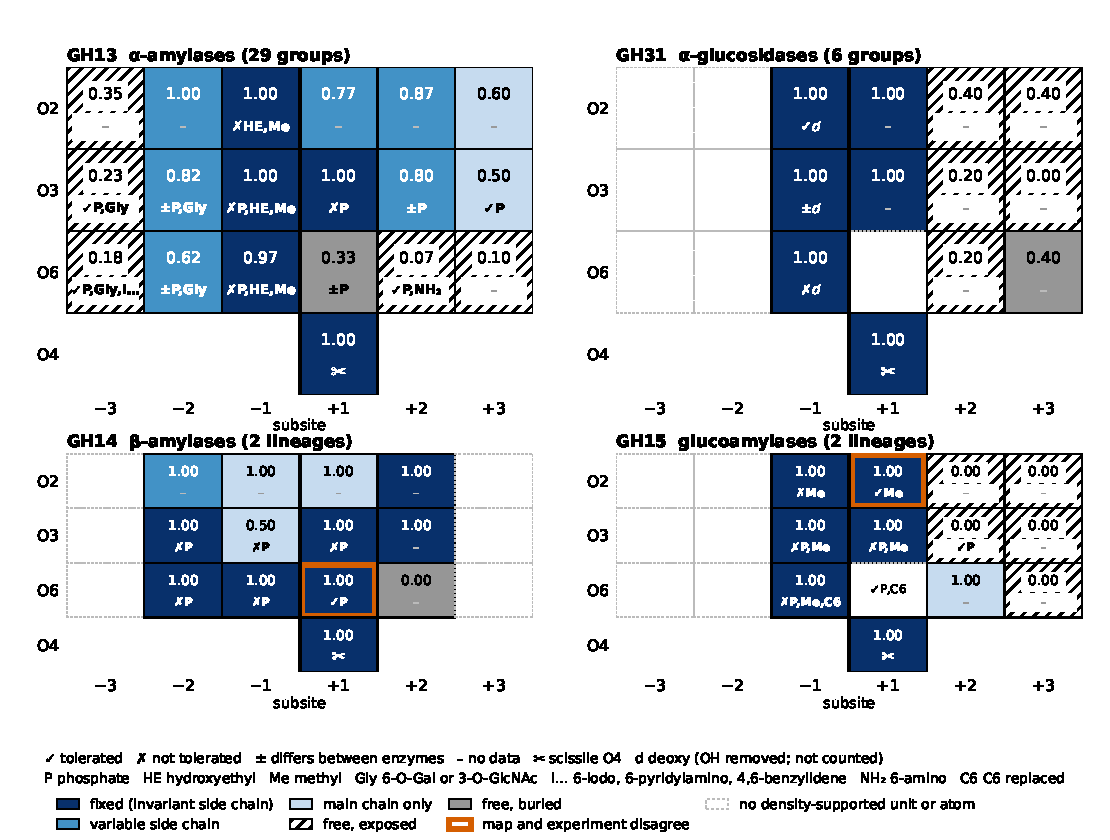
\includegraphics[width=\linewidth]{fig3_map.pdf}
\caption{The subsite $\times$ oxygen map. Cell colour, state of the oxygen
(Section~\ref{sec:methods_map}); number, fraction of 50\% sequence groups in which a protein N/O lies
within 3.5~\AA; lower mark, published result for a substrate substituted at that oxygen and
subsite (Table~\ref{tab:mapexp}). Bold line, the scissile bond. Source:
\texttt{45\_hydroxyl\_map/cell\_summary.tsv}.}
\label{fig:map}
\end{figure}

\begin{sidewaystable}
\centering\renewcommand{\baselinestretch}{1}\renewcommand{\arraystretch}{0.92}\scriptsize\setlength{\tabcolsep}{2pt}
\caption{The map against experiment, cell by cell. State and holding residues (reference
numbering: GH13 1AMY, GH14 1BYA, GH15 1AGM) from \texttt{45\_hydroxyl\_map/cell\_summary.tsv};
open surface in \AA$^2$ for EXP cells. Prediction: INV, not tolerated; EXP, tolerated; VAR,
depends on the enzyme. P, phosphate; HE, hydroxyethyl; Me, methyl. Ev.: FT, full text read;
ABS, abstract (\texttt{substituted\_starch\_hydrolysis\_literature.md}). Agreement: 19 of 21
cells with a prediction.}
\label{tab:mapexp}
\begin{tabular}{lllp{3.3cm}p{8.2cm}lp{4.2cm}}
\toprule
Fam. & Sub. & O & Map state (holding residues) & Experiment (substituent, enzyme, result) & Agree & Reference (Ev.)\\
\midrule
GH13 & $-3$ & O3 & EXP (26) & 3-P tolerated: \emph{A.~oryzae} and a bacterial liquefying $\alpha$-amylase & yes & \citep{Takeda1987} (FT), \citep{TakedaHizukuri1986,Kamasaka1997} (ABS)\\
GH13 & $-3$ & O6 & EXP (22) & 6-P tolerated: porcine pancreatic, \emph{A.~oryzae}; 6-iodo-6-deoxy: human salivary and pancreatic; 4,6-O-benzylidene favourable: porcine, human salivary & yes & \citep{Takeda1987} (FT), \citep{Takeda1983,Omichi1992,Kandra1997,Kandra2000} (ABS)\\
GH13 & $-2$ & O3 & VAR (Gln294 pos., Arg) & 3-P tolerated by \emph{B.~subtilis} and porcine; not by \emph{A.~oryzae} & yes & \citep{Takeda1987} (FT), \citep{Takeda1983,TakedaHizukuri1986} (ABS)\\
GH13 & $-2$ & O6 & VAR (Met52 pos.) & 6-P tolerated by \emph{B.~subtilis}; not by porcine, \emph{A.~oryzae} & yes & \citep{Takeda1987} (FT), \citep{Takeda1983,TakedaHizukuri1986} (ABS)\\
GH13 & $-1$ & O2 & INV (Asp289, Arg177, His288) & 2-O-HE not tolerated: porcine pancreatic & yes & \citep{Yoshida1984} (ABS)\\
GH13 & $-1$ & O3 & INV (Asp289, His288) & 3-O-HE, 3-P not tolerated: porcine, \emph{B.~subtilis}, \emph{A.~oryzae} & yes & \citep{Takeda1987} (FT), \citep{Yoshida1984,Takeda1983} (ABS)\\
GH13 & $-1$ & O6 & INV (Asp179, His92) & 6-O-HE, 6-P not tolerated: porcine, \emph{B.~subtilis}, \emph{A.~oryzae} & yes & \citep{Takeda1987} (FT), \citep{Yoshida1984,Takeda1983} (ABS)\\
GH13 & $+1$ & O3 & INV (Glu204) & 3-P not tolerated: all three $\alpha$-amylases & yes & \citep{Takeda1987} (FT), \citep{Takeda1983} (ABS)\\
GH13 & $+2$ & O3 & VAR (Lys182 pos.) & 3-P not tolerated by \emph{B.~subtilis}, porcine; tolerated by \emph{A.~oryzae} & yes & \citep{Takeda1987} (FT), \citep{Takeda1983,TakedaHizukuri1986} (ABS)\\
GH13 & $+2$ & O6 & EXP (27) & 6-P tolerated: \emph{B.~subtilis}; 6-amino-6-deoxy: human salivary and pancreatic & yes & \citep{Takeda1983,Omichi1992} (ABS)\\
\addlinespace
GH14 & $-2$ & O3 & INV (His93) & 3-P not tolerated: sweet-potato $\beta$-amylase & yes & \citep{Takeda1987} (FT)\\
GH14 & $-2$ & O6 & INV (Asp53, Arg420) & 6-P not tolerated: sweet-potato $\beta$-amylase & yes & \citep{Takeda1987} (FT)\\
GH14 & $-1$ & O6 & INV (Glu380, Lys295) & 6-P not tolerated: sweet-potato $\beta$-amylase & yes & \citep{Takeda1987} (FT)\\
GH14 & $+1$ & O3 & INV (Thr342) & 3-P not tolerated: sweet-potato $\beta$-amylase & yes & \citep{Takeda1987} (FT)\\
GH14 & $+1$ & O6 & INV (Glu186, Arg188) & 6-P tolerated: sweet-potato $\beta$-amylase & \textbf{no} & \citep{Takeda1987} (FT)\\
\addlinespace
GH15 & $-1$ & O2 & INV (Arg305) & 2-O-Me not tolerated: \emph{A.~niger} glucoamylase & yes & \citep{Lemieux1996} (ABS)\\
GH15 & $-1$ & O3 & INV (Arg54) & 3-O-Me, 3-P not tolerated: \emph{A.~niger} glucoamylase & yes & \citep{Takeda1987} (FT), \citep{Lemieux1996,Takeda1983} (ABS)\\
GH15 & $-1$ & O6 & INV (Asp55) & 6-O-Me, 6-P not tolerated: \emph{A.~niger} glucoamylase & yes & \citep{Takeda1987} (FT), \citep{Lemieux1996,Abe1982} (ABS)\\
GH15 & $+1$ & O2 & INV (Glu180) & 2-O-Me tolerated, kinetics virtually unaffected: \emph{A.~niger} glucoamylase & \textbf{no} & \citep{Lemieux1996} (ABS)\\
GH15 & $+1$ & O3 & INV (Glu180, Arg305) & 3-P not tolerated; 3-O-Me costs 1.9~kcal\,mol$^{-1}$ (25-fold in $k_\mathrm{cat}/K_\mathrm{M}$): \emph{A.~niger} glucoamylase & yes & \citep{Takeda1987} (FT), \citep{Takeda1983,Kamasaka1997,Lemieux1996} (ABS)\\
GH15 & $+2$ & O3 & EXP (30) & 3-P tolerated (one glucose left on the non-reducing side of the 3-P residue): \emph{A.~niger} glucoamylase & yes & \citep{Takeda1987} (FT), \citep{Takeda1983} (ABS)\\
\midrule
\multicolumn{7}{l}{Cells without a prediction}\\
GH13 & $+1$ & O6 & BUR (3 units) & 6-P tolerated by porcine, \emph{A.~oryzae}; not by \emph{B.~subtilis} & -- & \citep{Takeda1987} (FT), \citep{Takeda1983} (ABS)\\
GH13 & $+3$ & O3 & MC & 3-P tolerated: \emph{B.~subtilis}, porcine & -- & \citep{Takeda1987} (FT), \citep{Takeda1983} (ABS)\\
GH14 & $-1$ & O3 & MC & 3-P not tolerated: sweet-potato $\beta$-amylase & -- & \citep{Takeda1987} (FT)\\
GH15 & $+1$ & O6 & no O6 in the map & 6-P tolerated: \emph{A.~niger} glucoamylase & -- & \citep{Takeda1987} (FT), \citep{Takeda1983,Abe1982} (ABS)\\
\bottomrule
\end{tabular}
\end{sidewaystable}

\subsection{Whether substituents fit}\label{sec:fit}
\pend{substituent-fit analysis, \nolinkurl{resultados/analysis/46_substituent_fit/}}


\subsection{The rule is not carried by inhibitors or by repeated proteins}\label{sec:inhib}
This section and the next two use the 80\% selection of Section~\ref{sec:position}, counted per entry.
Many units at
$-1$ belong to acarbose-type inhibitors, which mimic the transition state rather than the
substrate. In GH13, the 24 entries whose labelled units are glucose only contact the six
positions contacted at $-1$ in at least 80\% of the entries (Asp179, Asp289, His288, Arg177,
His92, Tyr51) in 22--24 of 24, and the 50 inhibitor entries in 47--50 of 50; in GH31 the
glucose-only entries (5, from two proteins) contact all nine such positions (Asp327, His600,
Asp443, Asp542, Trp441, Trp539, Phe575, Ile328, Ile364) in 5 of 5. Nor is the count
made by a few proteins deposited many times: the 42 GH13 proteins fall into 29 groups at
50\% sequence identity and 5 at 30\%, across bacteria, archaea, fungi, plants and animals,
and each of the six $-1$ positions is contacted in at least 28 of the 29 groups and in all
5; the six GH31 proteins form 4 groups at 30\%, and the nine positions survive one vote per
group, Phe575 exactly at the 0.80 threshold.

\subsection{The rule is specific to the catalytic subsite}
Sugars also bind GH13 proteins
away from the catalytic cleft: 296 density-supported units lie more than 12~\AA{} from the
catalytic carboxylates and touch no position contacted at the subsites. These sites are mostly
particular to one protein; only 32 reference positions are contacted in at least four entries
from at least two proteins. Of the 15 whose side chains hydrogen-bond the sugar, all proteins
carry the same residue type at 7 (one vote per protein, 2--5 proteins per position). The
hydrogen-bonding positions of the GH13 catalytic subsite, sampled down to the same numbers of
proteins, carry a single residue type in 94\% of draws. A side chain that hydrogen-bonds a
sugar is fixed when it does so at the catalytic subsite, and only about half the time when it
does so elsewhere on the same proteins (aromatic positions away from the cleft: 1 of 7 fixed;
aliphatic: 3 of 7). Invariance is therefore not a property of binding a sugar as such; the
contrast is what a role in the transition state would produce.

\subsection{Families of other folds}\label{sec:folds}
GH13 and GH31 belong to different CAZy clans, GH-H and
GH-D, because their catalytic machinery differs, but a remote common ancestry of their
$(\beta/\alpha)_8$ barrels has been proposed~\citep{Janecek2007,Rigden2002}; they cannot show
whether the rule arose more than once. GH14 ($\beta$-amylase, an inverting enzyme in no
clan) and GH15 (glucoamylase, an inverting $(\alpha/\alpha)_6$ fold) can, within the limits
of their data. Counted per entry (80\% selection), in GH14 the side-chain hydrogen-bonders at $-1$ and $-2$ (Asp53, His93,
Arg420, the base Glu380, Lys295, the acid Glu186) and the aromatic Trp55 are invariant over
the 14--16 entries that contact them (Glu186 is contacted in 14 and hydrogen-bonds the sugar
in 10); the contacts at $-2$, the second ring of the two-glucose product, are made by
hydrogen-bonding residues. In GH15 the
hydrogen-bonders (Asp55, Arg54, the acid Glu179, Glu180, Arg305) and six aromatic residues
(Tyr48, Trp52, Trp317, Trp417, Trp120, Tyr311) are invariant over four entries. The
catalytic subsite of an unrelated fold is thus built from the same three kinds of residue.
The aliphatic residues of both families (GH14 Leu419, Leu20, Met17, Ala184; GH15 Leu177,
Leu415, Ala39) are also invariant, but each family has only two independent lineages
(GH14: barley and soybean, 66\% identical, and \emph{Bacillus cereus}, about 30\% to both;
GH15: three proteins, two fungal glucoamylases 34\% identical and a third whose UniProt
accession, Q12537, could not be resolved), too few for variation to show; neither the variability
of their aliphatic residues nor that of their outer-subsite ($-2$) hydrogen-bonders can be
tested there.

\subsection{Further observations at the same site}
Three observations from the same
structures and one calculation are given in the Supplementary material: the ring at
subsite $-1$ is distorted from the chair more often than at other subsites (Section~S1);
conserved water sites sit at the catalytic carboxylates of four families (Section~S2);
the computed pK$_\mathrm{a}$ of the catalytic residues differs between chains with and
without a bound ligand (Section~S3); and an MM/GBSA decomposition of four inhibitor
complexes of human lysosomal $\alpha$-glucosidase (Section~S4).

\subsection{The three kinds of contact differ in measured energy}
Kinetics with
deoxygenated substrates measure how much each sugar hydroxyl contributes to stabilising
the transition state, from $k_\mathrm{cat}/K_\mathrm{M}$ of the parent and the deoxy
analogue. For three GH13 yeast $\alpha$-glucosidases acting on methyl
$\alpha$-isomaltoside, each hydroxyl of the ring at $-1$ contributes 16.1--24.0~kJ\,mol$^{-1}$
and those of the ring at $+1$ at most 5.8~kJ\,mol$^{-1}$~\citep{Frandsen2002}; for a barley
GH31 $\alpha$-glucosidase, the $-1$ hydroxyls contribute 9.3--18.9~kJ\,mol$^{-1}$ and the
$+1$ 3-OH 7.0~kJ\,mol$^{-1}$~\citep{Frandsen2000}. Removing the residues that hydrogen-bond
these hydroxyls removes that energy and the activity with it: the barley $\alpha$-amylase~1
histidines His93 and His290 (His92 and His288 of the GH13 reference) lose 99\% of $k_\mathrm{cat}/K_\mathrm{M}$~\citep{Sogaard1993}, and the two
mutants of glucoamylase Arg54 -- an invariant hydrogen-bonder in our GH15 count -- lose
16--21~kJ\,mol$^{-1}$ of transition-state stabilisation, almost all of it in $k_\mathrm{cat}$,
with $K_\mathrm{M}$ between 25\% and 300\% of wild type~\citep{Frandsen1995}. Aromatic
contacts behave differently: replacing glucoamylase Trp120 by Phe lowers $k_\mathrm{cat}$
50-fold but leaves the hydroxyl energy profile of subsite $-1$ unchanged~\citep{Sierks2000},
and a sugar--aromatic contact is worth about 6~kJ\,mol$^{-1}$ in water, with many ring
orientations nearly equivalent~\citep{Asensio2013}. Across carbohydrate-binding proteins in
general, aliphatic residues are disfavoured in sugar pockets and aromatic ones
enriched~\citep{Hudson2015}. Read together with Table~\ref{tab:rule}, the
residues fixed in every lineage, the side-chain hydrogen-bonders of the rings at subsites
$-1$ and $+1$, are those whose contacts carry the large, measured transition-state energy;
aromatic contacts, smaller and permissive in orientation, keep an aromatic ring more often
than their identity; aliphatic contacts, with no specific role, change, as do contacts of
every kind at the outer subsites. The
kinetic data for the $\alpha$-enzymes come from $k_\mathrm{cat}/K_\mathrm{M}$ only and do
not separate transition-state from ground-state binding, as was done for a
$\beta$-glucosidase~\citep{Namchuk1995}; the GH13 hydroxyl values are for
$\alpha$-glucosidases on an $\alpha(1\!\to\!6)$ substrate, not for $\alpha$-amylases.

\subsection{A test the rule sets}
One of the non-catalytic GH31 positions of
Table~\ref{tab:rule} has a measured substitution: Asp327 of the reference is Asp404 of
human lysosomal $\alpha$-glucosidase, and the Pompe-disease variant Asp404Gly keeps the
protein level but leaves 3.6--6.6\% of normal activity in patient muscle~\citep{Nilsson2014}.
For His600, Trp441, Trp539, Phe575, Ile328 and Ile364 (their equivalents across GH31 proteins
fixed by structural alignment~\citep{Tan2010}) and for the aromatic Tyr51 of GH13 we found no mutant with
kinetic data (literature search, November 2026). The rule makes predictions for them:
replacing His600, which hydrogen-bonds the subsite $-1$ sugar, should cost transition-state
energy of the size measured for Asp404Gly and for the GH13 histidines; replacing Trp441 or Trp539 by Phe, or Tyr51 by Phe, should leave the hydroxyl
energy profile of subsite $-1$ largely unchanged, as for glucoamylase Trp120; and Ile328 or
Ile364 should accept Leu, Val or Met with little effect. These are the experiments that
would confirm the rule or break it.

\subsection{Design rules for processing functionalised starch}\label{sec:design}

\paragraph{(i) Substitution at O6 is better tolerated than at O2 or O3} In the GH13 map, O2 and O3
are held at five of the six subsites ($-2$ to $+3$, fixed at $-1$ and, for O3, at $+1$), and O6 at
two ($-2$ and $-1$), with O6 free and exposed at $-3$, $+2$ and $+3$ (Fig.~\ref{fig:map}). The
experiments with substituted starch point the same way: the 3-phosphate is excluded from more
subsites than the 6-phosphate by all three $\alpha$-amylases and by glucoamylase, which the
authors call more obstructive~\citep{Takeda1983,Takeda1987}; at equal content of unsubstituted
units, 2-O-hydroxyethyl starch resists porcine pancreatic $\alpha$-amylase more than
6-O-hydroxyethyl starch~\citep{Yoshida1973}; and hydroxyethyl starches with a higher C2/C6
substitution ratio are degraded more slowly in patients~\citep{Treib1995}. Our reading is that the
number of subsites at which an oxygen is held sets how many cuts near a substituted unit are
lost, so that a starch substituted mainly at O6 is hydrolysed further than one substituted at
O2 or O3 at the same degree of substitution. A 3-phosphate also restricts the conformation of
the adjacent glycosidic linkage~\citep{Hansen2009}, so part of the O3 effect may not come from
contact with the enzyme.

\paragraph{(ii) The choice of enzyme matters at subsites $-2$ and $+2$} In GH13, O2 and O3 at
$-2$ and $+2$ and O6 at $-2$ are held only by variable residues. The three $\alpha$-amylases
tested with phosphorylated glucan differ exactly there: \emph{B.~subtilis} $\alpha$-amylase
releases 6$^2$-phosphoryl maltotriose, placing a 6-phosphate at $-2$ and $+2$, whereas porcine
pancreatic and \emph{A.~oryzae} $\alpha$-amylases release 6$^3$-phosphoryl maltotriose, placing it
at $-3$ and $+1$; the 3-phosphate is accepted at $-2$ and $+3$ by the first two and at $-3$ and
$+2$ by the third~\citep{Takeda1983,TakedaHizukuri1986,Takeda1987}. The interpretation is that the
size and position of the products of a substituted starch are set by the residues at the
variable subsites of the enzyme chosen, while all three enzymes keep a substituted unit away
from $-1$ and from O3 at $+1$.

\paragraph{(iii) Engineering targets and positions to leave alone} The positions that hold O2,
O3 and O6 at $-2$ and $+2$ in GH13 already vary between lineages: the Gln294 position (Asp in
12 of 15 groups, Asn 2, Gln 1 in Table~\ref{tab:rule}), the Met52 position (Asp 9, Trp 5, Asn 3,
Gln 2, Gly 2, Phe 1) and the Lys182 position (Lys 9.5, Arg 2.5, His 2, Gln 1), all in the
reference numbering. Nature has exchanged their residues without losing the activity, which
makes them the first candidates for enzymes that accept a substituted unit at the outer
subsites. The residues that hold the oxygens at $-1$ and $+1$ are fixed in every lineage, and
their replacement is costly: the GH31 Asp327 position, which holds O4 and O6 at $-1$, is Asp404 of
human lysosomal $\alpha$-glucosidase, and its variant Asp404Gly leaves 3.6--6.6\% of normal
activity~\citep{Nilsson2014}; the GH13 histidines that hold O3 and O6 at $-1$ lose 99\% of
$k_\mathrm{cat}/K_\mathrm{M}$ when replaced~\citep{Sogaard1993}. These positions are off limits for
engineering towards substituted substrates.

\paragraph{(iv) Limits of the rules} The rules rest on 21 cells with experimental data; 18
of them include the products of one substrate, phosphorylated potato glucan, and 11 rest on it
alone. Of the phosphate sources only the review~\citep{Takeda1987} was read in full; the
hydroxyethyl and O-methyl results come from abstracts. No
subsite-resolved product study exists for hydroxypropyl, acetyl, octenyl-succinyl or
carboxymethyl starch, and none for GH31 with substituents bulkier than a deoxy change at
$-1$~\citep{Ogawa2004}. The two disagreements show that a fixed hydrogen bond in the crystal does
not by itself make an oxygen indispensable: O2 at $+1$ of glucoamylase is held by Glu180 but
contributes nearly nothing to the transition state~\citep{Lemieux1996,Bock1987}. Whether a given
substituent has room at a free oxygen is a separate question (Section~\ref{sec:fit}).

\subsection{What this does not show}
The fractions are properties of the deposited
structures, not binding affinities or populations in solution. Hydrogen bonds are assigned
from heavy-atom distances (and, in one test, heavy-atom angles), with no hydrogens placed, and aromatic stacking by residue type, not by ring geometry. The test
rests on 36 positions in GH13 and GH31 (Table~\ref{tab:rule}); GH14 and GH15 confirm the composition of the
site but not the variability of its aliphatic residues; GH57 (one protein) was not used.

\section{Conclusions}

Across hundreds of independently solved structures of starch-degrading glycoside hydrolases,
the side chains that hydrogen-bond the rings at subsites $-1$ and $+1$ are fixed in every
lineage, aromatic rings beside them are kept as rings, and aliphatic residues and residues of
every kind at the outer subsites change. Read atom by atom, this gives a design map for
functionalised starch: O2, O3 and O6 at $-1$ and O3 and the scissile O4 at $+1$ are held by
fixed residues and cannot carry a substituent; in GH13 the oxygens at $-2$ and $+2$ are held by
residues that vary between lineages, so tolerance there depends on the enzyme chosen; O6 and the
outer subsites are mostly free. The map agrees with published products and kinetics of
substituted substrates in 19 of 21 cells; the two exceptions, both at $+1$, are hydrogen bonds
that the kinetics show to be dispensable. Substitution at O6, enzymes chosen for their outer
subsites, and engineering at the variable $-2$/$+2$ positions rather than at the fixed
catalytic subsite follow from it.

\section*{CRediT authorship contribution statement}
\textbf{Aldo F. Combariza} (sole author): \pend{CRediT roles to be selected by the author from
the 14 CRediT roles}.

\section*{Declaration of competing interest}
\pend{statement of competing interests, to be made by the author}

\section*{Declaration of generative AI and AI-assisted technologies in the manuscript preparation process}
\pend{declaration to be written by the author (Elsevier template: tool used, purpose, extent of
oversight)}

\section*{Funding}
\pend{funding sources, or a statement that the work received no specific grant}

\section*{Data availability}
\pend{repository and DOI not yet decided}

\section*{Acknowledgements}
Computational resources and technical support were provided by the Laboratorio de
Supercomputaci\'on y C\'alculo Cient\'ifico (SC3) of the Universidad Industrial de
Santander (UIS), Colombia, through the GUANE high-performance computing cluster.

\section*{Appendix A. Supplementary material}
Supplementary material (Sections S1--S4, Tables S1--S3) accompanies this article
(ijbm\_SI.pdf).

\bibliographystyle{elsarticle-num}
\bibliography{ijbm}

\end{document}
